\documentclass{beamer}
\usepackage{graphicx}
\usepackage{tikz}
\usepackage{yquant}
\useyquantlanguage{groups}
\usepackage{pgfplots}
\usepackage{amsmath}
\pgfplotsset{compat=1.18}
\title{Qubit Movement-Optimized Program Generation on Zoned Neutral Atom Processors}
\author{Enhyeok Jang, Youngmin Kim, Hyungseok Kim, Seungwoo Choi, \textbf{Yipeng Huang}, and Won Woo Ro}
\institute{Yonsei University, Rutgers University}
\date{CGO ’25, March 01–05, 2025}

\begin{document}
	
	\frame{\titlepage}
	
	% Slide 1: Introduction
	\begin{frame}{Introduction}
		\begin{itemize}
			\item Zoned architectures improve gate fidelity ($>99.9\%$ for 1Q, $>99.5\%$ for 2Q).
%			\item However, inter-zone qubit movements take significantly longer than gate execution, leading to high execution overhead.
			\item Standard quantum program structures are inefficient on zoned architectures, requiring excessive zone-to-zone transfers.
			
		\end{itemize}
		\begin{figure}
			\centering
			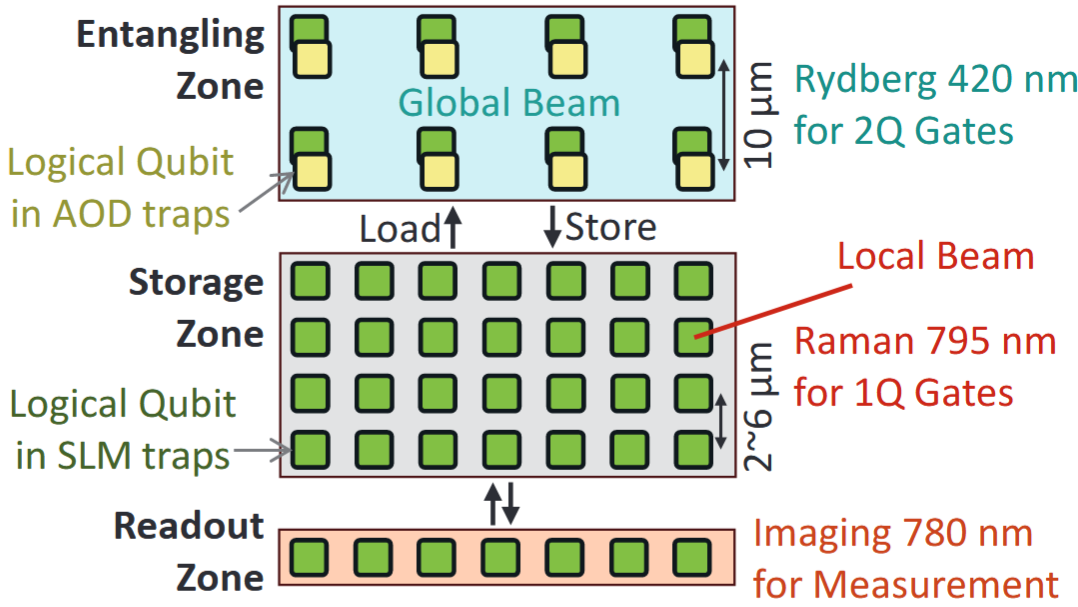
\includegraphics[width=.8\textwidth]{figure/zone.png}
			\caption{The entangling zone is dedicated to executing 2-qubit gates, while the storage zone is for single qubit gate.}
		\end{figure}
	\end{frame}
	
	% Slide 2: Motivation
	\begin{frame}{Motivation}
		\begin{itemize}
			\item Naïve program execution causes 78-89\% of runtime to be spent on zone-to-zone qubit transfers.
%			\item Gate structures such as CZ chains and ZZ interactions induce frequent interleavings of single- and two-qubit gates.
%			\item Existing neutral atom compilers do not sufficiently optimize inter-zone movements.
			\item \textbf{Goal:} Optimize program execution by reducing inter-zone qubit movements.
		\end{itemize}
		\begin{figure}
			\centering
			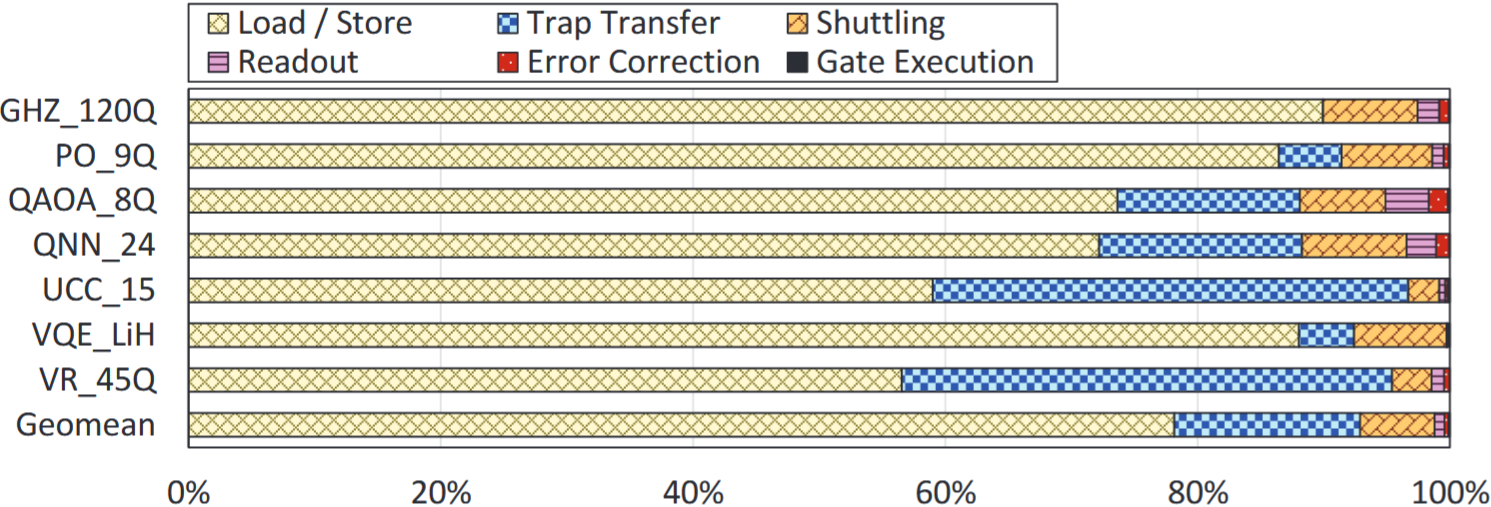
\includegraphics[width=.8\textwidth]{figure/intro.png}
			\caption{Execution time breakdown on zoned architectures.}
		\end{figure}
	\end{frame}
	
	% Slide 3: Mantra - Overview
	\begin{frame}{Mantra: Key Techniques}
		\textbf{Mantra (Minimizing trAp movemeNts for aTom aRray Architectures)} introduces:
		\begin{itemize}
			\item \textbf{Fountain-Shaped CZ Chain:} Reduces single-qubit gate overhead and cancels intermediate gates..
			\item \textbf{Preemptive Gate Scheduling:} Executes independent gates earlier to minimize inter-zone transitions.
			\item \textbf{1Q-Gateless ZZ Interaction:} Replaces CZ-based decompositions with direct Rydberg-mediated ZZ rotations
		\end{itemize}
		\textbf{Key Idea:} Reduces inter-zone movements and improves overall execution efficiency.
	\end{frame}
	
	% Slide 4: Fountain-Shaped CZ Chain
	\begin{frame}{Fountain-Shaped CZ Chain}
		\begin{itemize}
%			\item Standard chain structures cause excessive inter-zone movements due to alternating 1Q/2Q execution.
			\item Structure CZ chains around a common qubit.
		\end{itemize}
		\centering
		\begin{figure}
			\resizebox{!}{12ex}{
			\begin{tikzpicture}
				\begin{yquantgroup}
					\registers{
						qubit {} q[4];
					}
					\circuit{
						 cnot q[2] | q[3];
						 cnot q[1] | q[2];
						 cnot q[0] | q[1];
						 box {$Rz$} q[0];
						 cnot q[0] | q[1];
						 cnot q[1] | q[2];
						 cnot q[2] | q[3];
					}
					\equals
					\circuit{
						cnot q[0] | q[3];
						cnot q[0] | q[2];
						cnot q[0] | q[1];
						box {$Rz$} q[0];
						cnot q[0] | q[1];
						cnot q[0] | q[2];
						cnot q[0] | q[3];
					}
				\end{yquantgroup}
			\end{tikzpicture}}
		\caption[]{An example Hamiltonian simulation kernel $e^{-i\theta ZZZZ}$}
		\end{figure}
		\begin{figure}
			\resizebox{!}{12ex}{
				\begin{tikzpicture}
					\begin{yquantgroup}
						\registers{
							qubit {} q[4];
						}
						\circuit{
							h q[0];
							cnot q[1] | q[0];
							cnot q[2] | q[1];
							cnot q[3] | q[2];
						}
						\equals
						\circuit{
							h q[0];
							cnot q[1] | q[0];
							cnot q[2] | q[0];
							cnot q[3] | q[0];
						}
					\end{yquantgroup}
			\end{tikzpicture}}
			\caption[]{An example of a 4-qubit GHZ-state circuit.}
		\end{figure}
	\end{frame}
	
	% Slide 6: Preemptive Gate Scheduling
	\begin{frame}{Preemptive Gate Scheduling}
		\begin{itemize}
			\item Identifies independent gates that can be executed earlier in the same zone.
%			\item \textbf{Example:} GHZ state preparation.
			\item Reduces zone-to-zone movements while preserving computation dependencies.
		\end{itemize}
		\centering
		\begin{figure}
			\resizebox{!}{16ex}{
				\begin{tikzpicture}
					\begin{yquantgroup}
						\registers{
							qubit {} q[8];
						}
						\circuit{
							h q[0];
							cnot q[1] | q[0];
							cnot q[2] | q[0];
							cnot q[3] | q[0];
							cnot q[4] | q[0];
							cnot q[5] | q[0];
							cnot q[6] | q[0];
							cnot q[7] | q[0];
						}
						\equals
						\circuit{
							h q[0];
							cnot q[4] | q[0];
							
							cnot q[2] | q[0];
							cnot q[6] | q[4];
							
							cnot q[1] | q[0];
							cnot q[3] | q[2];
							cnot q[5] | q[4];
							cnot q[7] | q[6];
						}
					\end{yquantgroup}
			\end{tikzpicture}}
			\caption[]{An example of a 8-qubit GHZ-state circuit.}
		\end{figure}
	\end{frame}
	
	% Slide 5: 1Q-Gateless ZZ Interaction
	\begin{frame}{1Q-Gateless ZZ Interaction}
		\begin{itemize}
%			\item Standard implementations require interleaving 1Q and 2Q gates, causing frequent zone switching.
			\item \textbf{Mantra’s approach:} Uses a combination of adiabatic and Levine-Pichler gates to achieve direct ZZ rotations.
%			\item Eliminates the need for storage zone transitions during ZZ interactions.
		\end{itemize}
		\centering
		\begin{figure}
			\resizebox{!}{8ex}{
				\begin{tikzpicture}
					\begin{yquantgroup}
						\registers{
							qubit {} q[2];
						}
						\circuit{
							cnot q[1] | q[0];
							box {$RZ(\gamma)$} q[1];
							cnot q[1] | q[0];
						}
						\equals
						\circuit{
							box {$LP(\gamma)=
									\begin{bmatrix}
										1 & 0 & 0 & 0 \\
										0 & e^{-i\gamma} & 0 & 0 \\
										1 & 0 & e^{-i\gamma} & 0 \\
										1 & 0 & 0 & e^{2\gamma + \pi}
									\end{bmatrix}$} (q[0],q[1]);
							box {$Ad(\phi_1,\phi_2)=
								\begin{bmatrix}
									1 & 0 & 0 & 0 \\
									0 & 1 & 0 & 0 \\
									1 & 0 & 1 & 0 \\
									1 & 0 & 0 & e^{\phi_2 -2\phi_1}
								\end{bmatrix}$} (q[0],q[1]);
						}
					\end{yquantgroup}
			\end{tikzpicture}}
			\caption[]{The proposed arbitrary ZZ rotation protocol consisting of a single adiabatic (Ad) and a single Levine-Pichler (LP) gate, where $\phi_1 = (\pi+2\gamma+\phi_2)/2$.}
		\end{figure}
	\end{frame}

	
	% Slide 7: Results
	\begin{frame}{Results: Performance Improvement}
%		\begin{itemize}
%			\item Mantra reduces inter-zone movements by 68\%, leading to significant execution time savings.
%			\item .
%			\item Benchmarks (GHZ, QAOA, UCCSD, QNN) show up to 57-87\% reduction in execution time.
%		\end{itemize}
		\centering
		\begin{figure}
			\centering
			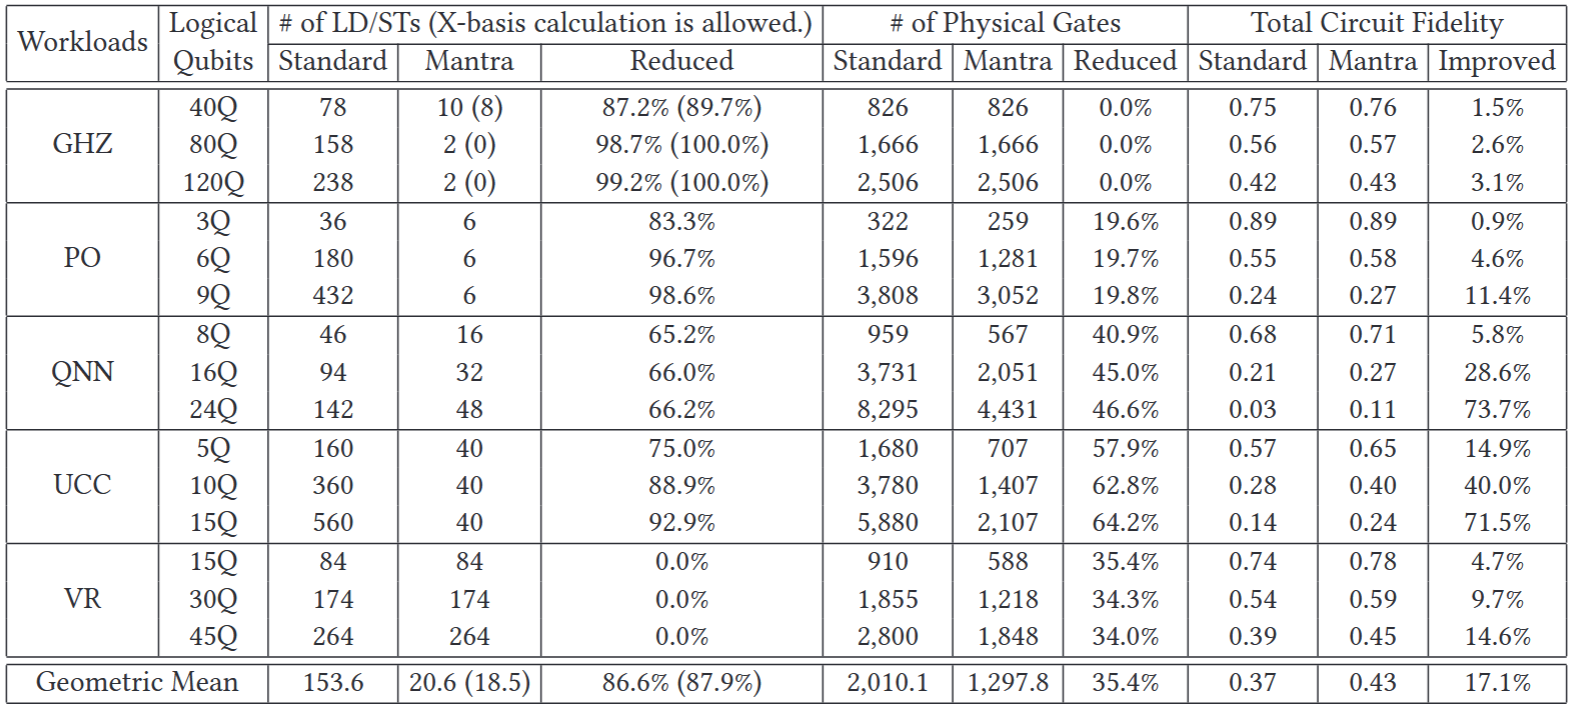
\includegraphics[width=.8\textwidth]{figure/res.png}
			\caption[]{Mantra reduces inter-zone movements by 86.6\%, also reduces physical gate counts by 35\%, improving overall fidelity by 17\%}
		\end{figure}
	\end{frame}
	
	\begin{frame}{Execution Breakdown According to Compiler}
		%		\begin{itemize}
			%			\item Mantra reduces inter-zone movements by 68\%, leading to significant execution time savings.
			%			\item .
			%			\item Benchmarks (GHZ, QAOA, UCCSD, QNN) show up to 57-87\% reduction in execution time.
			%		\end{itemize}
		\centering
		\begin{figure}
			\centering
			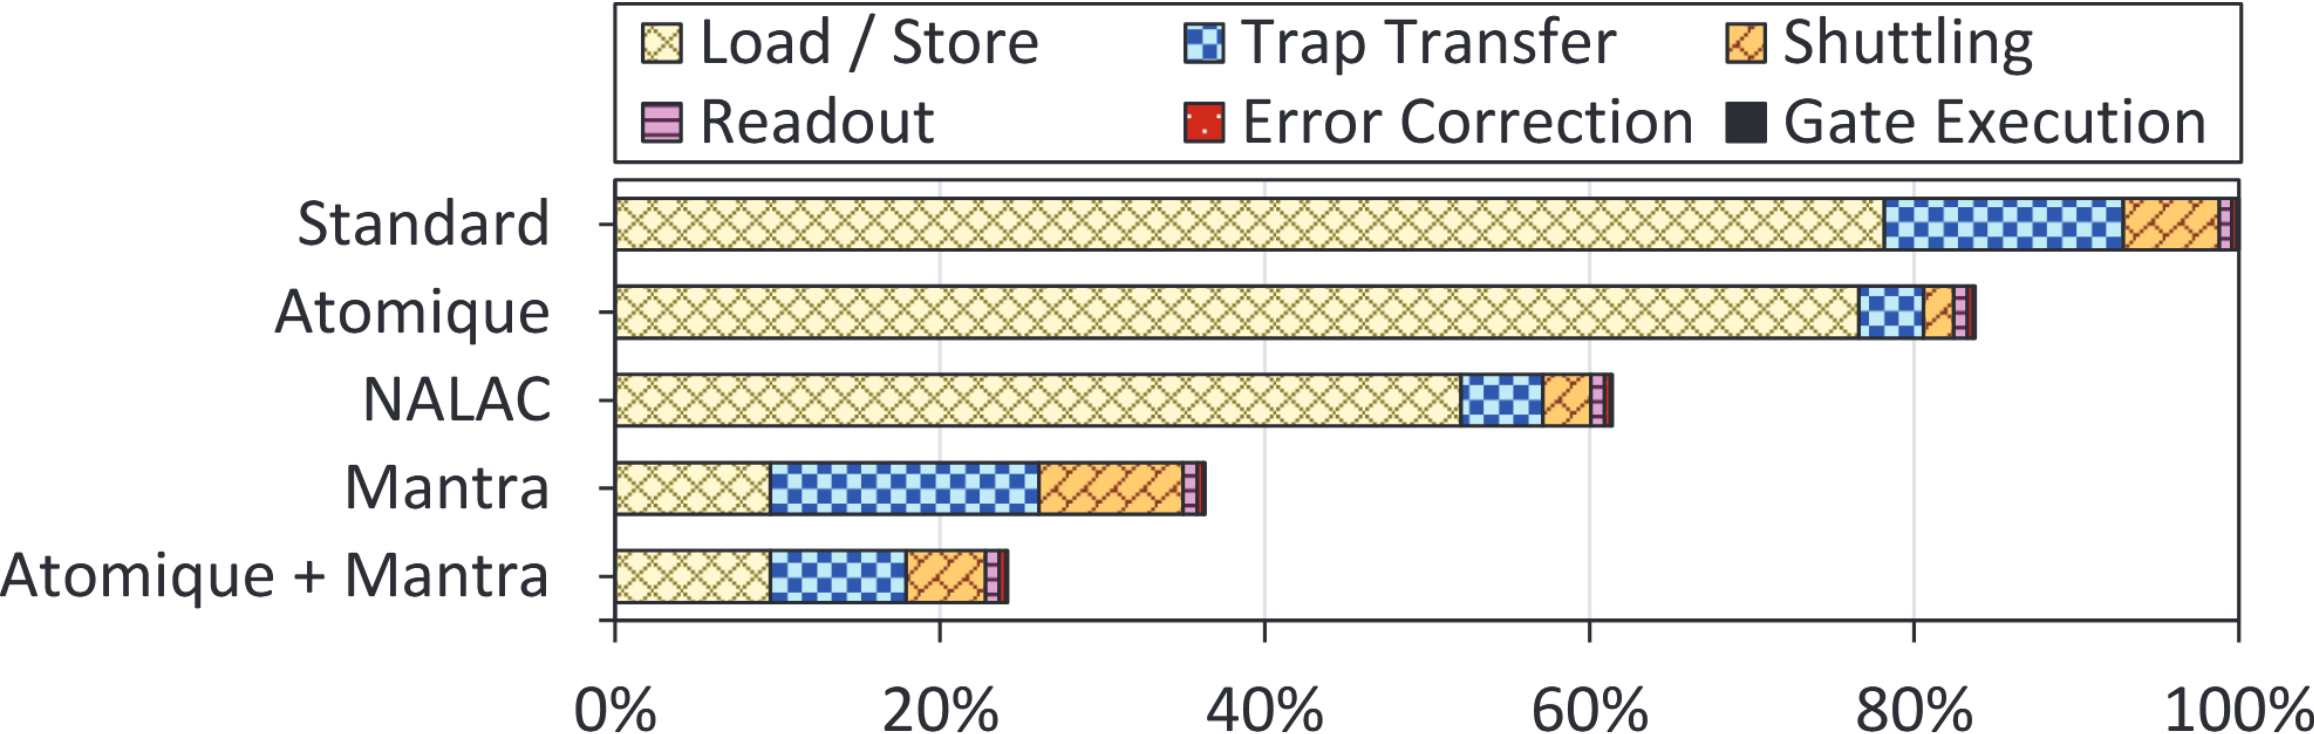
\includegraphics[width=.8\textwidth]{figure/different.png}
			\caption[]{Execution time breakdown analysis. Combining Atomique and Mantra could further enhance the performance of zoned architectures.}
		\end{figure}
	\end{frame}
	
%	% Slide 8: Discussion
%	\begin{frame}{Discussion and Future Directions}
%		\begin{itemize}
%			\item Zoned architectures are promising but require tailored compilation techniques.
%			\item Mantra improves execution efficiency by minimizing inter-zone movement overhead.
%			\item Future work: Extend optimization strategies for fault-tolerant quantum applications.
%		\end{itemize}
%	\end{frame}
	
	% Slide 9: Conclusion
	\begin{frame}{Conclusion}
		\begin{itemize}
			\item Zoned neutral atom architectures have high gate fidelities but suffer from slow qubit movement.
			\item Mantra optimizes execution by restructuring gate sequences and minimizing zone transfers.
			\item Results demonstrate significant reductions in execution time and improved fidelity.
%			\item These optimizations bridge the gap between algorithm design and hardware execution.
		\end{itemize}
	\end{frame}
	
\end{document}
